\documentclass[paper=a4, fontsize=11pt,twoside]{scrartcl}	% KOMA

\usepackage[a4paper,pdftex]{geometry}	% A4paper margins
\setlength{\oddsidemargin}{5mm}			% Remove 'twosided' indentation
\setlength{\evensidemargin}{5mm}

\usepackage[english]{babel}
\usepackage[protrusion=true,expansion=true]{microtype}	
\usepackage{amsmath,amsfonts,amsthm,amssymb}
\usepackage{graphicx}

\usepackage[utf8]{inputenc}

% use these packages for tables
\usepackage{booktabs}
\usepackage{tabu}
\usepackage{multirow}

% use for making captions beautiful
\usepackage[labelfont=bf, skip=5pt, font=small]{caption}

% package for color
\usepackage{xcolor}

% position images precisely at location in text
\usepackage{float}

% for algorithms
\usepackage{algorithm} 
\usepackage{algpseudocode} 



% --------------------------------------------------------------------
% Definitions (do not change this)
% --------------------------------------------------------------------
\newcommand{\HRule}[1]{\rule{\linewidth}{#1}} 	% Horizontal rule

\makeatletter							% Title
\def\printtitle{%						
    {\centering \@title\par}}
\makeatother									

\makeatletter							% Author
\def\printauthor{%					
    {\centering \large \@author}}				
\makeatother							

% --------------------------------------------------------------------
% Metadata (Change this)
% --------------------------------------------------------------------
\title{	\normalsize \textsc{Concordia University} 	% Subtitle
		 	\\[2.0cm]								% 2cm spacing
			\HRule{0.5pt} \\						% Upper rule
			\LARGE \textbf{\uppercase{Trigonometric function: \MakeLowercase{tan(x)}}}	% Title
			\HRule{2pt} \\ [0.5cm]		% Lower rule + 0.5cm spacing
			\normalsize \today			% Todays date
		}

\author{
		\textbf{\LARGE Arnab Roy} \\[10pt]
		{\Large Student Id: 40184043} \\[5pt]
		{\Large Team: E} \\
}


\begin{document}
% ------------------------------------------------------------------------------
% Maketitle
% ------------------------------------------------------------------------------
\thispagestyle{empty}		% Remove page numbering on this page

\printtitle					% Print the title data as defined above
\begin{center}
    \huge{Deliverable 1}
\end{center}
\vspace{35mm}
\printauthor				% Print the author data as defined above
\newpage
% ------------------------------------------------------------------------------
% Begin document
% ------------------------------------------------------------------------------
\tableofcontents
\newpage

\setcounter{page}{1}		% Set page numbering to begin on this page
\section{Introduction}
    The tangent function is one of the six trigonometric functions. It has many important uses in real life calculations such as calculating the slope of straight lines, angles of elevation and depression \cite{tanexamplewebsite1}, rate of altitude change of an aircraft \cite{tanexamplewebsite2} etc. \\
    The tangent function can be understood from an unit circle(a circle whose radius = 1).
    % inserting image of unit circle
    \begin{figure} [!h]
        \centering
        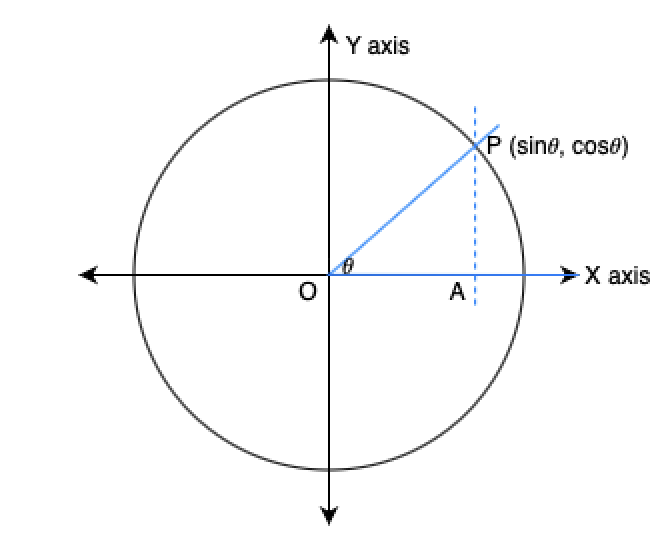
\includegraphics[width=0.4\textwidth]{Unit-circle.png}
        \caption{A unit circle}
        % labels help us to refer to within text and doesn't have any visual impact
        \label{fig:unit_circle}
    \end{figure} \\
    In a unit circle we take two lines originating from the center, one along the positive x axis and the other line intersecting the circumference of the circle. From the definition of unit circle, the coordinate of the point at which the circumference is intersected is $(\sin\theta, \cos\theta)$ \cite{unitcirclewebsite} and the tangent of the angle $\theta$ is:
    \begin{equation}
        \tan(\theta) = \sin(\theta) \div \cos(\theta) \label{tan_formula_1}
    \end{equation}
    \subsection{Domain and co-domain}
    The domain of $\tan \theta$ is x $\in \mathbb{R}$, x $\ne$ ($\pi$/2) + n*$\pi$ and its codomain is (-$\infty$, $\infty$) \cite{tandomainwebsite}.
    % inserting image of tangent graph
    \begin{figure} [H]
        \centering
        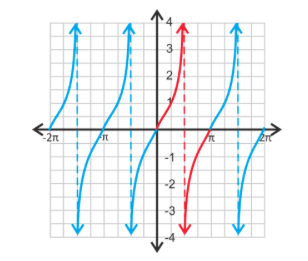
\includegraphics[width=0.4\textwidth]{graph-of-tangent.png}
        \caption{Graph of tangent function}
        % labels help us to refer to within text and doesn't have any visual impact
        \label{fig:graph_tangent}
    \end{figure} 
    \subsection{Interesting properties of the graph of the tangent function}
    The graph of the tangent function has some interesting properties. As cos$\theta$ = 0 when $\theta$ = $\pm$(n$\pi$/2) where n is odd, the graph approaches an asymptote along y-axis as cos$\theta$ approaches 0. Moreover, the graph has no amplitude and the period is calculated as the distance between any two high points or low points at the same height and the period is $\pi$. The graph intersects the y-axis only at (0,0) and the x-axis for $\theta$ = n$\pi$.
    
    \section{Requirements and assumptions for Tangent function}
The requirements and assumptions of the function tan(x) follow ISO/IEC/IEEE 29148 standards. A priority of 1 means most important and a priority of 5 means least important.
    \subsection{Assumptions}
    % defining a table
    % h! means put the table here. Latex will place the table to its liking by default. By h! we are commanding to put it right below the upper paragraph. Other options are b! and t! for bottom and top.
    \begin{tabular}{ |p{4cm} | p{10cm}| }
     \hline
     \multicolumn{2}{|l|}{\textbf{Assumption ID: F2-ASSUMP1}} \\
     \hline
     \textbf{Version:} & 1.0\\
     \textbf{Type:} & Functional\\
     \textbf{Owner:} & Arnab Roy\\
     \textbf{Priority:} & 1\\
     \textbf{Difficulty:} & Easy\\
     \textbf{Description:} & The user shall provide input in integers \\
     \textbf{Rationale:} & To keep the implementation simple and generate accurate outputs with a simple algorithm \\
     \hline
    \end{tabular}
    \\[10pt]
    \begin{tabular}{ |p{4cm} | p{10cm}| }
     \hline
     \multicolumn{2}{|l|}{\textbf{Assumption ID: F2-ASSUMP2}} \\
     \hline
     \textbf{Version:} & 1.0\\
     \textbf{Type:} & Functional\\
     \textbf{Owner:} & Arnab Roy\\
     \textbf{Priority:} & 1\\
     \textbf{Difficulty:} & Easy\\
     \textbf{Description:} & The user shall provide input in range -2$^{31}$ to 2$^{31}$-1 \\
     \textbf{Rationale:} & The range for the \texttt{int} primitive type is from -2$^{31}$ to 2$^{31}$-1 and to keep inputs small for a simple implementation\\
     \hline
    \end{tabular}
    \\[10pt]
    \begin{tabular}{ |p{4cm} | p{10cm}| }
     \hline
     \multicolumn{2}{|l|}{\textbf{Assumption ID: F2-ASSUMP3}} \\
     \hline
     \textbf{Version:} & 1.0\\
     \textbf{Type:} & Non-functional\\
     \textbf{Owner:} & Arnab Roy\\
     \textbf{Priority:} & 3\\
     \textbf{Difficulty:} & Easy\\
     \textbf{Description:} & The factorials for the calculation may be pre-stored in an array \\
     \textbf{Rationale:} & To speed up the calculation of the output and execution of the algorithm\\
     \hline
    \end{tabular}
    \subsection{Requirements}
    \begin{tabular}{ |p{4cm} | p{10cm}| }
     \hline
     \multicolumn{2}{|l|}{\textbf{Requirement ID: F2-REQ1}} \\
     \hline
     \textbf{Version:} & 1.0\\
     \textbf{Type:} & Functional\\
     \textbf{Owner:} & Arnab Roy\\
     \textbf{Priority:} & 1\\
     \textbf{Difficulty:} & Easy\\
     \textbf{Description:} & When the user enters a value for which cos(x)=0, an exception shall be thrown with an useful error message \\
     \textbf{Rationale:} & Tangent function does not have a valid output for angle=0 and the user shall be let known about this\\
     \hline
    \end{tabular}
    \\[10pt]
    \begin{tabular}{ |p{4cm} | p{10cm}| }
     \hline
     \multicolumn{2}{|l|}{\textbf{Requirement ID: F2-REQ2}} \\
     \hline
     \textbf{Version:} & 1.0\\
     \textbf{Type:} & Functional\\
     \textbf{Owner:} & Arnab Roy\\
     \textbf{Priority:} & 1\\
     \textbf{Difficulty:} & Easy\\
     \textbf{Description:} & If the output is -0.0, the function shall remove any signs and return 0.0 \\
     \textbf{Rationale:} & Using a sign with 0 is redundant and might be confusing to the user\\
     \hline
    \end{tabular}
    \\[10pt]
    \begin{tabular}{ |p{4cm} | p{10cm}| }
     \hline
     \multicolumn{2}{|l|}{\textbf{Requirement ID: F2-REQ3}} \\
     \hline
     \textbf{Version:} & 1.0\\
     \textbf{Type:} & Non-functional\\
     \textbf{Owner:} & Arnab Roy\\
     \textbf{Priority:} & 3\\
     \textbf{Difficulty:} & Medium\\
     \textbf{Description:} & The time complexity of the program should be in O(n) \\
     \textbf{Rationale:} & To keep program execution fast and within 1 second\\
     \hline
    \end{tabular}
    \\[10pt]
    \begin{tabular}{ |p{4cm} | p{10cm}| }
     \hline
     \multicolumn{2}{|l|}{\textbf{Requirement ID: F2-REQ4}} \\
     \hline
     \textbf{Version:} & 1.0\\
     \textbf{Type:} & Non-functional\\
     \textbf{Owner:} & Arnab Roy\\
     \textbf{Priority:} & 1\\
     \textbf{Difficulty:} & Hard\\
     \textbf{Description:} & All angles above 90 degree shall be converted within 90 degrees\\
     \textbf{Rationale:} & Calculation of smaller values is faster and all angles greater than 90 degrees can be converted within 90 degrees, so it is unnecessary to calculate higher values\\
     \hline
    \end{tabular}
    \\[10pt]
    \begin{tabular}{ |p{4cm} | p{10cm}| }
     \hline
     \multicolumn{2}{|l|}{\textbf{Requirement ID: F2-REQ5}} \\
     \hline
     \textbf{Version:} & 1.0\\
     \textbf{Type:} & Functional\\
     \textbf{Owner:} & Arnab Roy\\
     \textbf{Priority:} & 1\\
     \textbf{Difficulty:} & Easy\\
     \textbf{Description:} & The output of the function shall be a double\\
     \textbf{Rationale:} & Most outputs of tangents are in decimal and removing the fractional part would make the output inaccurate\\
     \hline
    \end{tabular}
    \\[10pt]
    \begin{tabular}{ |p{4cm} | p{10cm}| }
     \hline
     \multicolumn{2}{|l|}{\textbf{Requirement ID: F2-REQ6}}\\
     \hline
     \textbf{Version:} & 1.0\\
     \textbf{Type:} & Non-functional\\
     \textbf{Owner:} & Arnab Roy\\
     \textbf{Priority:} & 1\\
     \textbf{Difficulty:} & Medium\\
     \textbf{Description:} & The output of the tangent function shall be accurate upto 6 digits after the decimal\\
     \textbf{Rationale:} & Implementation of a simple algorithm has the trade-off of accuracy\\
     \hline
    \end{tabular}
    \\[10pt]
    \begin{tabular}{ |p{4cm} | p{10cm}| }
     \hline
     \multicolumn{2}{|l|}{\textbf{Requirement ID: F2-REQ7}}\\
     \hline
     \textbf{Version:} & 1.0\\
     \textbf{Type:} & Non-functional\\
     \textbf{Owner:} & Arnab Roy\\
     \textbf{Priority:} & 1\\
     \textbf{Difficulty:} & Medium\\
     \textbf{Description:} & The output shall be rounded to a value of 7 digits after the decimal\\
     \textbf{Rationale:} & Since the algorithm is accurate upto 6 decimal places and sometimes 7, the output would be rounded to 7 digits after the decimal\\
     \hline
    \end{tabular}
    \section{Algorithms}
\subsection{Pseudocode}
\subsubsection{The algorithm for sin(x)/cos(x)}
\begin{algorithm}[H]
	\caption{tangent(angle) using sin(angle)/cos(angle)} 
	\begin{algorithmic}[1]
		\State result = calculateSin(angle)/calculateCos(angle)
		\If {result is equal to $\infty$}
		\State throw error
		\EndIf
		\State Round result to 7 digits
        \State \textbf{return} result
	\end{algorithmic} 
\end{algorithm}

\begin{algorithm}[H]
	\caption{calculateSin(angle)} 
	\begin{algorithmic}[1]
		\State convert angle to 360 degrees
		\If{angle is less than 0}
		    \State store the sign of angle
		    \State angle = absolute value of angle
		\EndIf
		\State determine the quadrant of the angle
		\State signInQuadrant = calculate the sign of the angle in determined quadrant
		\State shouldSubtract = true
		\State angleInRadian = angle * 3.141592654 / 180
		\State squareOfRadianAngle = angleInRadian * angleInRadian
		\State numerator = angleInRadian * angleInRadian * angleInRadian
		\State digitToFactorial = 3
		\State result = angleInRadian
        \For{$i=1\ldots9$}
         \State nTerm = numerator / factorials[digitToFactorial]
         \If{shouldSubtract}
            \State nTerm *= -1
            \State shouldSubtract = false
            \State \textbf{else}
            \State shouldSubtract = true
        \EndIf
        \State result += nTerm
        \State numerator = numerator * squareOfRadianAngle
        digitToFactorial += 2
        \EndFor
        \State result = roundTo7Digits(result)
        \State \textbf{return} result == 0 ? 0 : result * sign * signInQuadrant
	\end{algorithmic} 
\end{algorithm}

\begin{algorithm}[H]
	\caption{calculateCos(angle)} 
	\begin{algorithmic}[1]
        \State convert angle to 360 degrees
        \If{angle is less than 0}
            \State angle = absolute value of angle
        \EndIf
        \State determine the quadrant of the angle
		\State signInQuadrant = calculate the sign of the angle in determined quadrant
        \State shouldSubtract = true
        \State angleInRadian = angle * 3.141592654 / 180
        \State squareOfRadianAngle = angleInRadian * angleInRadian
        \State numerator = squareOfRadianAngle
        \State digitToFactorial = 2
        \State result = 1
        \For{$i=1\ldots9$}
            \State nTerm = numerator / factorials[digitToFactorial]
            \If{shouldSubtract}
                \State nTerm *= -1
                \State shouldSubtract = false
            \State \Else
                \State shouldSubtract = true
            \EndIf
            \State result += nTerm
            \State numerator = numerator * squareOfRadianAngle
            \State digitToFactorial += 2
        \EndFor

        \State result = roundTo7Digits(result)
        \State \textbf{return} result == 0 ? 0 : result * signInQuadrant
	\end{algorithmic} 
\end{algorithm}

    \subsubsection{The algorithm for the Taylor series of tangent function}
    \begin{algorithm}[H]
    	\caption{tangent(angle) using Taylor series} 
    	\begin{algorithmic}[1]
            \State nominator[13] = [1, 1, 2, 17, 62, 1382, 21844, 929569, 6404582, 443861162, 18888466084, 113927491862, 58870668456604]
            \State denominator[13] = [1, 3, 15, 315, 2835, 155925, 6081075, 638512875, 10854718875, 1856156927625, 194896477400625, 49308808782358125, 3698160658676859375]
        \State result = 0
        \State squareOfAngle = angle * angle
    
        \For{$test=0\ldots12$}
            \State result += angle * nominator[test] / denominator[test]
            \State angle *= squareOfAngle
        \EndFor
        \State \textbf{return} result
    	\end{algorithmic} 
    \end{algorithm}
    \subsection{Description of the implemented algorithm}
    We have implemented the tangent function using the sin/cos formula. For this, we need the Taylor series for sine and cosine. At first, the angle in degrees provided by the user is converted within 90 degrees and the quadrant is determined. The it is converted to radians. The algorithm considers upto 9 terms and achieves an accuracy upto 6 decimal digits.
    \subsubsection{Time complexity}
    O(N)
    \subsubsection{Space complexity}
    O(T), where T is the number of factorials generated.
    \subsection{The advantages and disadvantages}
    We have implemented the tangent(angle) using the sin(angle)/cos(angle) algorithm. It has several advantages of the Taylor series of the tangent function. To understand this, we will first discuss about the disadvantage of the Taylor series of tangent.
    \subsubsection{Disadvantage of Taylor series of tangent}
    \begin{itemize}
        \item The algorithm is not accurate for smaller terms. A large number of terms (approximately 30) needs to be taken to get an accurate result.
        \item The denominator of the 13th term of the series is 3698160658676859375. It is evident that the denominators of the larger terms will exceed the capacity of the primitive data types in Java.
        \item Keeping the Taylor series small results in output whose fractional parts are largely deviated from the accurate result.
    \end{itemize}
    \subsubsection{Advantage of sin(x)/cos(x)}
    \begin{itemize}
        \item Needs only 9 terms for the Taylor series of sine and cosine to make the output accurate upto 6 fractional parts
        \item Smaller number of terms mean faster execution
    \end{itemize}
    
    \section{Information about the debugger used}
    For the purpose of debugging the method written for calculating the tangent of an angle, the Intellij IDEA debugger was used. This debugger comes pre-bundled with the Intellij IDEA IDE. This makes coding and debugging streamlined.
    \subsection{Advantages}
    Using a pre-bundled IDE comes with many advantages, one of which is ease of debugging when writing code. Some of the capabilities that this debugger provides is:
    \begin{itemize}
        \item Shows the variables and their updated values for each line of code. Values are shown in the code inline for each variable and also all variables and values are shown in the variables window.
        \item Allows jumping to variable, variable type and method declaration.
        \item Allows changing variable values during debugging, change program flow and execute conditional code branches.
        \item Allows evaluation of complex code expressions on the fly.
        \item Enables pausing the debugging procedure and check the call stack and the running threads.
        \item Enables setting breakpoints on lines. The debugger stops code execution at the breakpoint and the user can manually execute the remaining code statements, one by one.
        \item Allows dragging a breakpoint and dropping it on another line to move a breakpoint from one line to another. Also allows setting multiple breakpoints and disabling them.
        \item Enables setting conditional breakpoints, where the application is stopped at that line if a certain condition is met.
        \item Allows stepping over a method, stepping into a method or stepping out of a method during debugging. JDK methods are stepped over by default and the focus is towards user written methods and statements.
        \item Enables “run to cursor” feature, where the debugger does not stop at lines until the one at which the mouse cursor is at.
    \end{itemize}
    \subsection{Disadvantages}
    The debugger is very resource intensive. It can easily slow down a machine with 8GB RAM and Intel Core i7 processor for very large programs.
    \section{Effort to make the program better}
    When writing the program, focus was given to make it correct, efficient, maintainable, robust, and usable. An explanation of the steps taken to make them such is given below.
    \subsection{Correctness}
    According to the requirements, the program needs to be correct up-to 6 decimal digits of a Casio scientific calculator. The result of the tangent function in the program depends on the results of the sine and the cosine functions. These functions were implemented using the Taylor series and severals steps were taken to increase their accuracy. 
    \begin{itemize}
        \item At first, only 3 terms from the Taylor series were considered, which later was increased to 9. The inclusion of more terms  increased the accuracy but was not enough.
        \item It was observed that for smaller angle values, the calculations were very accurate. But for higher values, the results started to deviate. So, all angles were first converted within 360 degrees. 
        \item To further increase the accuracy, they were converted to 90 degrees and the quadrant was calculated to determine the sign (+ or -) of the result. This also eliminated a problem during calculation of cosine of 180 which outputted 1.0000008 instead of 1.
        \item For many calculations, Java shows -0. These results were checked so that the output for 0 does not have any sign.
    \end{itemize}
    \subsection{Efficiency}
    To calculate the tangent of an angle, the Taylor series algorithm was implemented which is a O(n$^2$) algorithm because of the calculation of the factorials for each term. To make it efficient, the values of the factorials were calculated beforehand at once and stored in an array. To calculate the factorial of n, n was multiplied with the value of (n-1)th index in the array and the result was stored at nth index of the array. This algorithm takes place in O(n) time and the values can be accessed in O(1) time. Thus the run time complexity of the algorithm was reduced to O(n) and the space complexity increased to O(n). The rounding function runs in O(1) time complexity.
    \subsection{Maintainability}
    To make the program maintainable, the lines of code were properly documented by comments. Most code, which would be repeatable and reusable, were separated into separate small functions. The methods return appropriate error messages. The code was written in a way so that it is easier to read and meaningful variable names were used.
    \subsection{Robustness}
    For the tangent function, one pitfall is when the value of cosine is 90 degrees. For this case, an \texttt{ArithmeticException} was thrown with an error message that could be clearly understood by the user.
    \subsection{Usability}
    The functions written for the tangent, cosine and sine functions do not have input prompts themselves. They require driver programs to take the input from the user and pass it as arguments. The output and error messages from the tangent function notifies the user about the result as a clearly understandable string.
    \section{Unit Testing Guidelines}
    \begin{itemize}
        \item Each test case has a small description
        \item Test case have been designed mapping them to the functional requirements
        \item Test cases have been assigned unique IDs
        \item Each test have the name of the method that are tested
        \item Test cases are elaborate
        \item All corner cases have been tested
    \end{itemize}
    \section{Description of Checkstyle}
    For this project, an extension of Checkstyle for IntelliJ IDEA had been used. The source code was analyzed with the Google style. It generated 121 warnings, most of which were related to code indentation. It suggested a tab width of 2 spaces instead of 4. This type of indentation makes the code clearer to read. Moreover, another type of warning was to comment before classes and methods using JavaDoc. It also warned about comments that are more than 100 words long on a single line. \\
    The advantages of using CheckStyle is that it enforces strict coding conventions which is useful across teams. The code analysis was also very fast. \\
    One disadvantage of the extension was that, it did not show the errors inline, like most static source code analysers do.
    
    \section{Code review of \Gamma(x)}
    \subsection{Purpose}
    The purpose of this review is to check whether the quality of code in the module is degrading the quality of the system, i.e the Calculator app. Some standard guidelines have been followed to review the code. 
    \subsection{Guidelines}
    For this code review, the Google developer guidelines which is available at https://google.github.io/eng-practices/review/reviewer/looking-for.html have been followed. The guidelines are as follows:
    \begin{itemize}
        \item Check whether the code components interact well with other code components.
        \item The code functionality satisfies the users
        \item Outputs from error messages are well written and articulated
        \item Naming conventions for functions, variables, classes are good and communicate well to the user
        \item The code has unit tests that are maintainable and not complex
        \item The code has well written comments that add value and are not too lengthy
        \item The code follows a style guide
        \item The code is not over engineered
        \item No unnecessary import statements have been used
    \end{itemize}
    \subsection{Approach}
    Several approaches were followed when reviewing the code and they are as follows:
    \begin{itemize}
        \item The code was read through and it was identified whether the naming conventions were good and whether the comments were useful and did not exceed 100 characters per line. Effort was given to check whether any function war too large and whether it needed breaking down into smaller functions.
        \item The code was run using a debugger line by line. The return values and error messages were checked against the requirements.
        \item The test cases were run to check if all had passed. It was also checked whether the test cases had clearly understandable assertions. 
        \item It was checked whether the code followed a consistent style.
    \end{itemize}
    \subsection{Results of review}
    \begin{tabular}{ |p{7cm} | p{7cm}| }
     \hline
     \textbf{Attribute} & \textbf{Result}\\
     \hline
     \textbf{Code component interaction:} & PASS\\
     \textbf{Correct functionality:} & PASS\\
     \textbf{Clear error messages:} & PASS\\
     \textbf{Naming convention:} & PASS\\
     \textbf{Unit tests:} & PASS\\
     \textbf{Useful comments:} & PASS\\
     \textbf{Style guide:} & PASS\\
     \textbf{Code base not too complex:} & PASS\\
     \textbf{No unnecessary imports:} & PASS\\
     \hline
    \end{tabular}
    
    \subsection{Conclusion}
    The code-base of this module had all the necessary quality attributes. My only suggestion would be if in some small places, the coding styles would not be neglected, for example for the spacing around curly braces.
    
    \section{Testing the ab$^x$ function}
    The author of the function provided all the unit tests which were done using the JUnit library. Since we had a difference in the development environment, at first I was facing some issues with the JUnit library configuration. After resetting the configurations, JUnit worked correctly. \\
    At first I individually ran the test cases for various types of input. They all passed. Finally, I ran the test class all together and that passed as well.\\
    The IDE I was using was IntelliJ IDEA and I had JUnit 5 installed along with Juniper as dependencies. The OS I am using is MacOS 11.5.
    
    \bibliographystyle{ieeetr}
    \bibliography{bibliography}

% ------------------------------------------------------------------------------
% End document
% ------------------------------------------------------------------------------
\end{document}